\documentclass[a4paper, 12pt]{book}
\usepackage{natbib}
\usepackage{amsmath}
\usepackage{amssymb}
\usepackage{amsfonts}
%\usepackage{epstopdf}
\usepackage{graphicx}
\usepackage{epstopdf}
\usepackage{adjustbox}
\usepackage[table]{xcolor}
\usepackage[toc, page]{appendix}

% Drawing
\usepackage{tikz}
\usetikzlibrary{matrix}
\usetikzlibrary{shapes,arrows}

% Expectation symbol
\DeclareMathOperator*{\E}{\mathbb{E}}

% Cool titles
\usepackage{sectsty}
\allsectionsfont{\sffamily}

\begin{document}
\tableofcontents

\newpage

% Introduction 
\chapter{Introduction}


Radars have several highly attractive properties: they are active systems independent on lighting conditions, are very fast and have high precision. Furthermore, implemented at millimeter-wave wavelengths, radar sensors can be designed as low-power devices with no moving parts in a favorable form factor \citep{lien_gillian_karagozler_amihood_schwesig_olson_raja_poupyrev_2016}.

Radar technology has been around since the 1930s \citep{watson-watt_1945}, and has since developed into a well established field of engineering. Although the archetypal use case in radio-frequency (\gls{rf}), radars regard detection and tracking of large objects at far distances, such as for air and marine monitoring, new areas of applications have emerged under recent years posing very different engineering challenges. Some of these are outlined in \citep{amin_2017}, where close-range radars are used for applications such as vital signs monitoring \citep{kuo_lin_yu_lo_lyu_chou_chuang_2016}, gesture recognition \citep{lien_gillian_karagozler_amihood_schwesig_olson_raja_poupyrev_2016} and tumour imaging \citep{klemm_gibbins_leendertz_horseman_preece_benjamin_craddock_2011} to name a few. Furthermore, millimeter-wave radars have lately become more inexpensive, largely due to their widespread adoption in the automotive industry \citep{frenzel_2018}, making such devices an attractive option in a wide range of low cost applications.

Alongside the miniaturization of radar systems a trend in data science has emerged; the movement towards machine learning centric methods. This transition, spanned over multiple decades, has placed machine learning as an increasingly popular choice for data analysis. Machine learning algorithms encompass a very large set of algorithms, but fundamentally utilize various statistical techniques in order to allow computer systems to progressively improve performance \citep{a_smola_svn_vishwanathan_2010}. Data scientists have found machine learning, which forms a subclass of aritficial intelligence, particularly practical for data that lack an easily predictable structure.

In this work we investigate whether millimeter-wave radar can be used for surface recognition. Two broad antenna beams illuminate a target scene, and using a feature extraction procedure and machine learning techniques the returning echo is analyzed in order to classify the surface type. This work focuses on the use case of determining if a surface is grassy or not, but could easily be extended to invoke other surface types as well.  

\section{Motivation and previous work}

Autonomous robots have found increasing use in numerous devices, from helping customers navigate stores \citep{mcsweeney_2018} to keeping floors clean \citep{sanfacon_2017} and mowing lawns \citep{udelhofen_2018}. A common challenge with such systems is keeping the robot in bounds. This commonly means for the robot to be aware where on a two-dimensional map it is currently located. In certain applications however, "in bounds" rather involves staying on one type of material, such as autonomous robot lawn mowers staying only on areas covered in grass, or robot vacuum cleaners on regions without a carpet. In such devices one may be content with knowing that the robot roams around remaining on its designated surface type rather than having knowledge of its exact position. 

Surface classification can also be used in autonomous devices as a supporting system. A robot vacuum cleaner could for instance make use of such a system in numerous ways, such as for avoiding liquid spills or using surface-dependant cleaning programs. One could easily imagine other use cases where such a system would be a great convenience.

In order to distinguish one surface type from another some feature of the surface at hand must somehow be captured and analyzed. This very general problem statement can and has been approached from many different angles.

Taking inspiration from the recent advances in computer vision, one may be tempted to use cameras for visual inspection of the surface at hand. Computer vision has indeed attracted extensive research over the past few decades with impressive results \citep{liu_chen_fieguth_zhao_chellappa_pietikäinen_2018}. In a computer vision framework, images of different surfaces can be separated by their differences in \emph{texture} - their spatial organization of basic elements. Such fundamental microstructures obey some kind of statistical properties which can be percepted by for instance a convolutional neural network. Effective texture identification of textures in image databases was used in, for example, \citep{do_vetterli_2002} for accuracte classification. 

Although using computer vision for accurate real time target identification is an attractive option, it is commonly an infeasible option for small devices with limited hardware capabilities. Cameras capture light in the visible frequency spectrum, which inherently renders them sensitive to changes in light conditions. Thus, unless direct illumination of the target surface is used, solutions involving cameras are highly dependent on ambient light. Such a limitation can make cameras impractical for small devices navigating areas with varying lighting.

The perhaps most immediate way to perform surface identification is through direct contact. In \citep{giguere_dudek_2011}, surface identification for low-velocity mobile robots using a small metallic rod with an attached accelerometer. By capturing accelerometer output induced in the tip of the rod during robot motion identification was possible for a couple of different surface types. While probing may produce appealing results in certain situations, the method is fundamentally based on physical contact with the target. Hence, a probe is more susceptible to damage, can more easily get stuck and is more exposed to detrimental tear over time than its non-interfering counterparts.

% Two chief methods for doing this - Ultrsonic and radar. 
For surface classification with devices in motion, the seemingly two chief non-contact methods researchers have spent their time on for this application are ultrasonic methods and radar-based methods. These two methods are both noninvasive and have modest power requirements. Furthermore, both are active systems and thus do not need to rely on any ambient signal source. Ultrasonic and radar systems have been tested by researchers for road condition monitoring \citep{bystrov_2016}, \citep{mckerrow_kristiansen_2006}. 

These two methods primarily utilize the difference in roughness, a geometric characteristic of a surface caused by spatial variations in surface depth. Researchers experimenting with ultrasonic sensors (perhaps motivated by a study proving bats capable of discriminating surfaces with different roughness with their echolocation \citep{schmidt_1988}) have found some degree of success. In \citep{politis_probert_1999} angled ultrasonic sensors were used to measure roughness. By comparing the distribution of energy between specular (i.e. mirror-like) and diffuse componenets of ultrasonic echo they were able to distinguish between six different surface types, and modeling the floor as having a random structure on the form of a Gaussian distribution around the surface plane creating. Using this method the researchers were able to generate predictions on a sample-by-sample basis, not taking the temporal dimension into account.
% Work with the last part here - radar applications/radarCat etc. We wish to utilize time-based methods. Would be neat to find radar work doing nearly the same thing. Finally - we are using a single recieving antenna.

\begin{figure}
	\centering
	\includegraphics[scale=0.8]{figs_temp/acc_sensor}
	\caption{Image of the 60 GHz PCR radar sensor used in this work. Image retrieved from \emph{www.acconeer.com/products}.}
	\label{fig:acc_sens}
\end{figure}


\section{Objective}

In this work, we seek to create a model capable of performing binary surface classification from data collected during robot movement. By collecting data on grass surfaces and selection of non-grass surfaces we wish to create an effective classifier able to distinguish a grass covered surface from other surface types. All experiments will be performed using two 60 Ghz pulsed coherent radar \gls{pcr} sensors from Acconeer, see figure \ref{fig:acc_sens},  mounted on the front of device moving straight at a constant velocity. 

\section{Thesis outline}

The oulline of this thesis is as follows:
\\ \\
\noindent\textbf{Chapter 2:} This chapter explains the fundamentals of \gls{pcr} systems, as well as describe how distance, reflectivity and radial velocity can be extracted from the radar response. 
\\ \\
\noindent\textbf{Chapter 3:} In chapter 3 we proceed with describing the method used for collecting the data used in this project. Sensor settings, such as pulse length and sampling frequency, are discussed. 
\\ \\
\noindent\textbf{Chapter 4:} Chapter 4 presents the feature extraction process for surface identification. Temporal features, such as the autocorrelation function and the fourier transform, are investigated for accurate surface classification. At the end of the chapter, one of the tested extraction methods is selected for further investigation. 
\\ \\
\noindent\textbf{Chapter 5:}  In this chapter, some different classfiers are tested for prediction accuracy. Both linear and non-linear machine learning models are tested. At the end of the chapter, one machine learning classifier is found to be the best. 
\\ \\
\noindent\textbf{Chapter 6:} In chapter 6 some postprocessing and optimizations to the best found model are discussed. 
\\ \\
\noindent\textbf{Chapter 7:} Chapter 7 examines the found models capabilities in real and artificially created test scenarios. The found results are discussed, and some limitations are discussed.
\\ \\
\noindent\textbf{Chapter 8:} In chapter 8 conclusions of this work is presented and possible directions of future work is discussed. 







%In spite of their rise in populatity, solutions for surface classification using high frequency radars are somewhat scarce. When a single radar sensor is used for this purpose and a nonstationary setting is considered such as for a device moving across a surface of interest, very little previous work can be found in litterature. The perhaps closest resemblance is the RadarCat project\citep{yeo_2016}. As a part of Google's project Soli, RadarCat used a radar sensor for material classification. Nonetheless, a central part of this approach was having an object stationary and in direct contact with the radar sensor. The focal point of Project Soli was gesture recognition. This application bears some similarities to surface classification in motion in the regard that the subject is nonstationary. However classifying surfaces during motion and classifying hand gestures differ on a critical point - gestures are actions performed during some window in time while a robot moving along a surface is a continuous operation. 



%Continue: You want to be able to do this on a budget.


%\subsection{Previous work}


%It is in many applications of interest to obtain images of subsurface identification nondestructively. In recent decades, ground penetrating radar (GPR) has found increasing use in evaluation of road conditions \citep{solla_gonzález-jorge_varela_lorenzo_2013} for preservation and maintenance of infrastructure.


%A major challenge in radar sensing is to not only detect, but also to identify radar targets. This can for example be used for monitoring of urban environments \citep{harter_kowalewski_sit_jalilvand_ziroff_zwick_2014}.


%Localization is the classic use-case for radars. 
%\\ \\
% Radar  can detect relatively small targets at near or far distances and can measure their range with  precision  in  all weather,  which is  its chief  advantage when compared with other  sensors \citep{skolnik_2009}
%\\ \\
%Radar classification: 


% Classifying underground objects - this is a good paper we should look deeper into
%Using a ground penetrating radar (GPR), it is possible to identify subsurface objects. 
%Significantly lower frequency (900 MHz)
%\citep{lu_pu_liu_2014}.
% Paper on ground penetrating radar
%\citep{daniels_2004}

% RadarCat


%Chapter 3: Mention something about the data collecting process. Motive our choice of parameters such as sampling frequency. Go through visual observations of our data.

%Chapter 4: Feature selection and preprocessing is considered. Signal structure is discussed primarily on an intuitive level. 

%Chapter 5: Classification schemes. Moving from simple to advanced, some classifiers of special interest are investigated. Results with regards to these classifiers are presented.

%Chapter 6: Disucssion.

%Chapter 7: Conclusion.


% Radar system overview
\chapter{Radar system overview}


In order to build a model capable of accurately capturing key features from various areas one must first understand the origin of the received signal. In this chapter a few fundamental concepts in radar systems are introduced considered critical for understanding the radar responses produced in the measurement setup outlined in the previous chapter. First, the basic principles of radar is explained. The manner in which electromagnetic waves disperse and scatter in a space are briefly discussed. Then, some important features in an actual radar system are considerd. These involve how the radar transmits its wavelets, the mixing process of returning waves and the demodulation procedure used for accurate phase tracking. 

\section{The radar principle}

\subsection{Fundamental concepts}

The radar principle is at its core simple. A radar operates by radiating electromagnetic energy and detecting the echo returned from reflecting targets in its field of view. By examining properties of the echo signal it is possible to obtain information about the targets is provided. This may involve the range at which scatterers are located, the angular at which targets are found or the speed at which a scatterer moves. With a sufficiently high angular and range resolution it is also possible to discern parts of the targets size and shape. 


Radars are active systems, meaning that it radiates using its own antenna and does not depend on ambient radiation . 

\citep{skolnik_2009}


A wavelet pulse $x_T(t)$ with some carrier frequency $\Omega$  is transmitted towards an object of interest. After some short time $t_1$, the radar listens for an echo. If no echo is received, it means there is no object present at distance\footnote{The reason for dividing by 2 is that the wavelet pulse must first travel from the radar to the object, and then find its way back to the radar.}
\begin{equation}
	d_1 = \frac{v_0\cdot t_1}2
\end{equation}
where $v_0$ is the speed of an electromagnetic wave in air. After the previously transmitted wavelet is guaranteed to have died out, a new one is transmitted. Again, the radar listens for an echo, but this time after another time $t_2$ has passed. $t_2$ is greater than $t_1$, meaning the radar listens for echoes further away. If an echo is received, it means there is an object present at distance 
$
	d_2 = \frac12(v_0\cdot t_2).
$
This process is repeated for different time delays $t_i$. The chosen time delays can be adjusted depending on in what ranges one wants to search in, and how good range resolution one seeks.

Together, the echoes (or lack thereof) from each transmitted wavelet make up one sweep. A sweep is often plotted in an amplitude-vs-range, or amplitude-vs-depth diagram as in figure (...). This plot is a good way to visualize at what ranges objects are present.

* Plot of sweep *

\subsection{Radar wave dispersion}

How signals get weaker by a factor 1/r4

1-dimensional data: signals propagate in a spherical manner

How this ties in to what we do


If it is assumed that the radar pulses are transmitted isotropically, and no power is lost in the transmission medium, the power density at a range $R$ is the emission power $P_t$ divided by the surface area of a sphere with radius $R$.

\begin{equation}
	P(R) = \frac{P_t}{4\pi R^2}
\end{equation}


In this report a singular radar transmitter and receiver is used. 



\citep{skolnik_2009}, \citep{richards_2014}


\section{Radar operation}

A pulsed radar system can be realized in countless ways, but all subscribe to the fundamental physical laws of electromagnetic radiation. In this section one such configuration is described. Furthermore, we describe the key signal processing method, \emph{In-phase and Quadrature-phase demodulation} (IQ demodulation), used for extracting useful information from the unprocessed radar response. 

\subsection{Elements of a pulsed radar}
The radar system considered in this report includes the following crucial components:

\begin{itemize}
	\item Waveform generator
	\item Oscillator
	\item Transmitting antenna
	\item Receiving antenna
	\item Mixer
	\item Integrator
\end{itemize}

% List of parts in radar system
% Nice figure showing this process


A waveform generator outputs a radar envelope which is modulated by a local oscillator to some desired radio frequency. After signal amplification the wavelet is transmitted through an antenna. Detection is performed by a second antenna, which receives the returning signal during some time interval. 

\subsection{Mixing}

After receiving the returning radiation the signal then goes through a process known as \emph{mixing}. An internal wavelet is generated at a very specific delay from the initial pulse transmission and multiplied with the received signal. If the received and internal pulses do not match, the output of this multiplication will be zero. If there however exist some overlap between the internal and returning signals the output will be nonzero, indicating some level of energy content at the distance corresponding to the internal pulse delay. By increasing the internal pulse delay and repeating this procedure a set of measurement points is obtained. Mixing is thus achieved by multiplying a large number of returning wavelets with internally generated wavelet counterparts, adding a slight delay between sampling points. 

% Describe why this process is equivalent to an autocorrelation
% Include plot of raw data to show what a real sweep looks like.

Figures \ref{fig:mix0}, \ref{fig:mix1} and \ref{fig:mix2} illustrate this principle. In the upper plot in the first two figures two analysis wavelets are shown, each at a different time delay. The center plot show the received radar pulse registrered by the antenna, and the lower plot the result when the two above signals are multiplied elementwise. Note that the final figure show the result of multiple received electromagnetic pulses, each sample point representing a summation of one set of multiplications between returning and internally generated signals. This output will henceforth be called the \emph{raw signal}.   

\begin{figure}[h]
	\centering
	\includegraphics[scale=0.5]{figs_temp/mixing0}
	\caption{Analysis pulse (top), received pulse (mid) and multiplication output (bot). As the signals do not overlap the multiplication yields only zero values.}
	\label{fig:mix0}
\end{figure}

\begin{figure}[h]
	\centering
	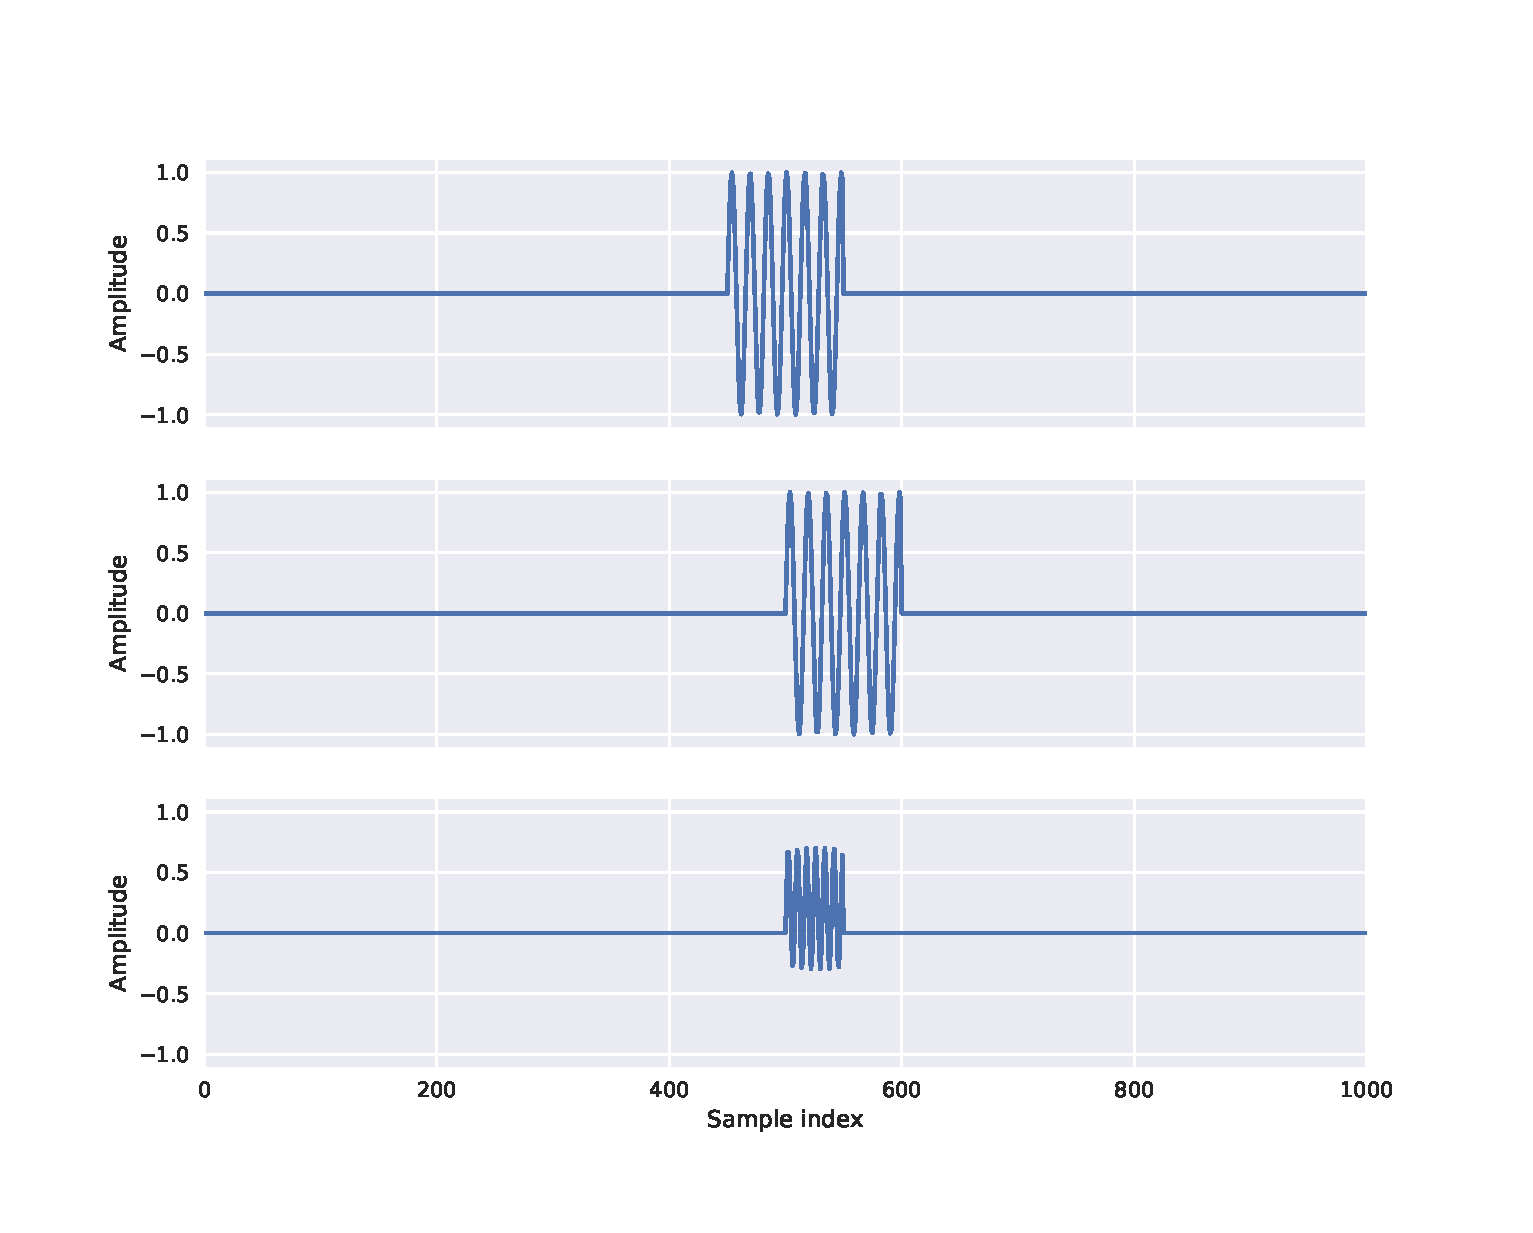
\includegraphics[scale=0.5]{figs_temp/mixing1}
	\caption{Analysis pulse (top), received pulse (mid) and multiplication output (bot). The overlapping signals produce varying amplitudes at the output sensitive to small changes in phase.}
	\label{fig:mix1}
\end{figure}

\begin{figure}[h]
	\centering
	\includegraphics[scale=0.5]{figs_temp/mixing2}
	\caption{By integrating the multiplication at each delay the mixing output is produced.}
	\label{fig:mix2}
\end{figure}



\subsection{IQ demodulated data}
A common type of data when working with radar signal processing is in-phase and quadrature-phase data (IQ-data).  This type of data is useful in that it contains information not only about amplitude, but about the phase of the radar signal as well \citep{richards_2014}. IQ-data is represented as complex numbers, and a radar sweep consists of several such complex numbers - one for each investigated range. To obtain the amplitude plot, as the one in figure .... for a sweep, $s$, made up of IQ-data, one simply computes the absolute value for each complex number in $s$. Similarly, a phase curve can be obtained by computing the phase in each point. A phase curve can typically look like the one in *Figure of phase plot*

In many applications, the phase information in IQ-data is used when small changes in the radar signal need to be detected, (Mention a case such as recording over grass...) as the phase is more sensitive to changes than the amplitude \citep{lien_gillian_karagozler_amihood_schwesig_olson_raja_poupyrev_2016}. If an object is detected at distance $r(t_1)$ from the radar at time $t_1$, and shortly thereafter, the object is moved to distance $r(t_2)$, the corresponding difference in phase will be
\begin{equation}
	\label{eq:phase_diff}
	\Delta\phi(t_1, t_2)=\frac{4\pi}{\lambda}(r(t_2)-r(t_1)) \quad\quad \textrm{mod 2$\pi$}
\end{equation}
By having a sampling frequency which is too low, the range difference in $\eqref{eq:phase_diff}$ could potentially become very big, and the phase difference would fluctuate over time and be incomprehensible.

In the case of material classification, a high sampling frequency is highly beneficial. When moving across surfaces characterized by tiny details, a high sampling frequency is essential in capturing the shape of these.

For a thorough description of how IQ-data is derived from raw radar data, we refer to \citep{richards_2014}

\chapter{Data}
\section{Data Collecting}
Having reliable data is a fundamental requirement in building a good model. There are many parameters to consider in optimizing the data collecting process. However,  finding an optimal solution is often impossible as the combinations are endless, but putting some thought into every decision often proves worthwhile. Below, we motivate our choices of sensor placement as well as various parameters.

\subsection{Measurement Setup}


Include graphics of the sensor placement etc. and describe the setup briefly. Possibly mention the $\frac14\lambda$ gap between the sensor and RLM plastic.
\subsection{Measurement Settings}
Having reliable data is a fundamental requirement in building a good model. Hence, choosing suitable parameters such as sampling frequency, regions of interest and planning a good measurment setup are all crucial tasks. The sampling frequency is particularly important to consider when working with means that could potentially cause aliasing. One such case is the DFT \citep{lindgren_rootzeŽn_sandsten_2013}. If the sampling frequency is too low, we get aliasing etc. etc. 

In order to assure that aliasing is avoided, the maximal frequency component registered by the radar must be surpassed by half the sampling frequency
\begin{equation}
	f_{max} < \frac{f_s}{2}.
\end{equation}
The sampling frequency can be chosen accordingly, assuming the maximal frequency component is known. 

In figure (fig. from previous subsubsection) a vehicle is moving forward with constant speed, having a sensor mounted at the front. As it moves forward, small objects on the ground get closer to the radar sensor with some speed. This gives rise to a doppler frequency being registered by the radar, which is \citep{lien_gillian_karagozler_amihood_schwesig_olson_raja_poupyrev_2016}
\begin{equation}
	f_{d} = \frac{2v_\perp}{\lambda}.
\end{equation}
...


\section{Data exploration}

Good source on PCA
\cite{hyvasrinen_karhunen_oja_2004}
PCA 125-143

Information theory
105-122
Argument for downsampling in range: In an information theoretic framework we interpret a random variable by how unpredicable or unstructured an observation of the variable is. This concept, examining the randomness of a variable, is commonly measured through entropy. Directly related to entropy is mutual information which essentially is how much information each member of a set have on the other members. \cite{hyvasrinen_karhunen_oja_2004}. Ideally one wants measurements that have a low measure of mutual information, meaning that each datapoint contain information not found elsewhere in the set. 

Observing a typical radar sweep[ref to plot with sweep] we note that points are very closely related on a small range scale, and nearly identical if we were to examine them on a sample by sample basis. One could argue that the mutual information found in the set is very high and that the entropy in each datapoint is low. Hence, to lower the first and increase the latter, one could downsample by some factor $D$ in range without significant loss of information.


PCA 125-143: Through the point and feature selection methods described in previous sections we obtain high dimensional feature vectors. Getting an intuitive feel for such data extracted in these processes is difficult as direct plotting is limited to three dimensions. 

Principal Component Analysis (PCA) is  a classical technique in statistical data analysis which takes a large set of multivariate variables and finds a smaller set of variables with less redundancy. Critically, PCA finds a rotated orthogonal coordinate system such that the elements of the set become uncorrelated. Projecting elements on the principal axes corresponding to the directions of maximal variance a good approximation of the original data in lower dimension is obtained \citep{hyvasrinen_karhunen_oja_2004}. 


% Data acquisition and preprocessing
\chapter{Data Preprocessing}
\section{Downsampling}
Add reference to Information Theoretic part

Since the correlation between neighboring range samples is very high we can downsample without significant loss of information. The downsampling process essentially requires three hyperparameters: A starting range $R_{start}$ and an end range $R_{end}$ where we begin and end our downsampling process respectively, as well as a downsampling factor $D$.

\begin{equation}
	x_D(n, t) = x(R_{start} + nD, t) \quad \text{for}\quad n=0...\frac{R_{end}-R_{start}}{D}
\end{equation}

\section{Sweep Normalization}
The gain of Acconeer radars can vary significantly from one sensor to another. Despite facing towards the very same surface, two sensors may exhibit a similar sweep structure,  yet with very different amplitudes. This could potentially have serious consequences if not handled properly. Assuming measurements for a model's training data have been collected with one sensor, it would be impossible to successfully perform classifications with a sensor which has a very different gain. The recordings would simply have too little resemblence, even though they merely differ by a constant gain factor.

A way to combat this problem is to perform some kind of sweep normalization before proceeding with any other preprocessing. There are numerous ways of doing this. A rather simplistic strategy could be to simply normalize each sweep with its maximum value. While this may intuitively seem like a good idea, it may erroneously normalize sweeps which contain outliers (Is this really a problem? What is it really that makes this method work bad?)

A more robust solution is to compute the average energy of ...

Explain normalization procedure: divide all sweeps within a feature box with the total energy within that feature box. 

Mention this was the best approach, but do not go into detail about the other methods - if so, just mention them briefly.


% Feature selection
\chapter{Feature selection}

In order to create an effective predictive model one must first select a set of features used to produce each classification. Both a science and an art, this process involves intuition, theory and a hefty amount of trial-and-error. Although a seemingly daunting task, for a model to be effective the feature selection procedure is key, and a carefully considered selection often generates significantly better results than one hastily put together. 

Ideally, one seeks a small set of variables which accurately captures the information content in a larger set of data. After reducing the number of features into a more manageable format it is then possible to obtain good results with significantly less computational load than if no feature selection had been considered. Furthermore, the feature selection process allows us to pinpoint what data characteristics we wish to monitor, and subsequently which data characteristics we can disregard. 

\section{An impossible problem}

Fundamentally, the radar used transmits pulses with some envelope $A(t)$ of some frequency $\Omega$ into its surroundings.

\begin{equation}
	x(t) = A(t)\sin(\Omega t + \varphi)
\end{equation}

After scattering, a signal $s(t)$ reaches the receiving antenna. This signal is comprised of radiation diffuesly scattered from the target scene. It contains both specular (i.e. mirror-like) and non-specular reflective components. Its content will be a function dependant both on the surrounding surface topography, as well as the dielectric properties of the surface at hand \citep{grossman_popovic_chamberlin_gordon_novotny_2017}. Furthermore, the surfaces at hand have a, to some degree, random structure with varying properties. The great difficulty with modeling $s(t)$ is clear - the universe of all possible "realistic" surfaces, both natural and man-made, is almost impossibly large. And since we in the present case are unable to make any significant assumptions with regards to the surface landscapes tested, there is no real useful model of $s(t)$ we can make. Instead, we have to come up with a set of \emph{reasonable} features that \emph{should} capture the signal structure. Hence our task is to find \emph{defining characteristics} from a given surface using the sequence of one dimensional data obtained from a radar sensor. 

The reflectivity of a material, described by its dielectric constant, shows up in the obtained IQ-demodulated sweeps in the amplitude of the returning signals. Therefore it might seem like a good idea to simply measure the energy content of a sweep and use it as a feature. However, due to inconsistencies inbetween individual sensors sweep normalization is performed as a pre-processing step rendering such calculations unusable. We are thus left with investigating the topography of the scene. 

As the radar samples rather quickly at around 200 Hz we can allow ourselves to use a sequence of sweeps to generate one prediction. This allows for feature-processing over a number of sweeps, rather than on a sweep-by-sweep basis. Besides improving the signal-to-noise ratio \citep{w_doerry_2016} we may also investigate time correlations when using multiple radar sweeps. If $T$ sweeps are used per classification, the rate of classifications $F_c$ produced relates to the sampling rate $F_s$ through

\begin{equation}
	F_c = \frac{F_s}{T}
\end{equation} 
The parameter $T$ becomes a tradeoff between accuracy and classification rate. The more samples $T$ used per classification the higher the classification accuracy is at the cost of a lower classification frequency. Conversely we may be able to generate feature estimates more rapidly by setting $T$ to a lower value, but will in the process end up with worse feature estimates. 

\section{Features}

In this section four different features are discussed aimed at capturing the geometric characteristics of a target surface. A radar datapoint captured at time $t$ and range $n$ is denoted as $x(n,t)$. Since we are using $T$ samples per classification, each new set of features $f_m$ are estimated from time $t_m=Tm$ to $Tm+T-1$ 

\subsubsection{Expected signal}

First of all we may characterize a sweep by its envelope form - that is, the shape of the absolute values of the radar sweeps. For range $i$ and feature index $m$, $T$ consecutive samples are averaged over to yield the averaging estimate $s_i(m)$ through

\begin{equation}
	s_i(m) = \frac{1}{T}\sum_{t=0}^{T-1}|x(i, t_m + t)|.
\end{equation}

\begin{figure}[h]
	\centering
	\includegraphics[scale=0.7]{figs_temp/features/sweep_average}
	\caption{By averaging a number of consecutive sweeps, we reduce noise and make samples more similar. The dashed line shows the average of the solid lines. }
	\label{fig:sweep_average}
\end{figure}

\subsubsection{Autocovariance - range}


We can regard the sequence $\{x(i,t)\}_{t=t_m}^{t_m+T}$ of measurements of range $i$ as samples from a stochastic process $X_{i,t}$ with the autocovariance function

\begin{equation}
	C_{XX}(i,t_m,s) = \text{Cov}(X_{i,t_m},X_{i,s}).
\end{equation}

If we then can consider the process to be having the following three properties:
\emph{
\begin{enumerate}
	\item Constant finite mean
	\item Autocovariance function only dependant on the difference $(s-t)$ and not on actual values of $s$ and $t$.
	\item Finite variance
\end{enumerate}
}
over the time interval $t_m$ to $t_m+T-1$, it can be regarded as a \emph{Wide-Sense Stationary} (WSS) process \citep{jakobsson_2015}. The first and second assumptions require the returning signal to carry some level of stability, which is reasonble considering the short time-frame $T/F_s$ considered. From the autocovariance function 

\begin{equation}
	r_i(m, k) = \E\big\{(X_{i,t_m} - \E\{X_{i,t_m}\})^*(X_{i,t_m+k} - \E\{X_{i,t_m+k}\})\big\}
\end{equation}

we can then form the (biased) estimated autocovariance function through

\begin{equation}
	\hat{r}_i^b(m, k) = \frac{1}{T}\sum_{t=0}^{T-1-k}\big(x(i,t_m+t) - s_i(t_m)\big)^*\big(x(i,t_m+t+k) - s_i(t_m)\big)
\end{equation}

\subsubsection{Autocovariance - energy}

We can also calculate the autocovariance function of estimated sweep energy. Although the sweeps are normalized in the preprocessing, we can investigate how the sweeps change over time. 

The average energy in a sweep tells us how much energy is reflected back to the radar. Hence it can be regarded as a measure of how good of a reflector the underlying surface is. The energy depends on the shape of the surface, as well as its dielectric constant. Compared to other materials, grass has a very different surface shape, which potentially gives it a very different reflexivity. However, its dielectric constant could also vary a lot depending on whether it is wet or dry, making it hard to guess its reflective properties.

By computing the average energy of single sweeps from different surfaces we see in figure \ref{fig:sweep_energy} that grass reflects much less energy. This indicates that the average sweep energy is a good feature for binary grass/not grass classification. However, in order to get a more robust measure of the average energy we do not only compute the average over selected range bins of a single sweep, but we average over a few consecutive sweeps as well. Mathematically, the feature we end up using becomes
\begin{equation}
	P(t_m) = \frac{1}{NT}\sum_{t=0}^{T-1}\sum_{n=0}^{K-1}x(n, t_m + t)x^*(n, t_m + t),
\end{equation}
where (describe variables)

Despite the fact that the average energy appears to be a highly relevant feature, it is also much gain dependent, and conflicts with what is stated in section *reference to sweep norm.*. Therefore, if different sensors are to be used for training and future classifications, this feature will not be of any use.

\begin{figure}[h]
	\centering
	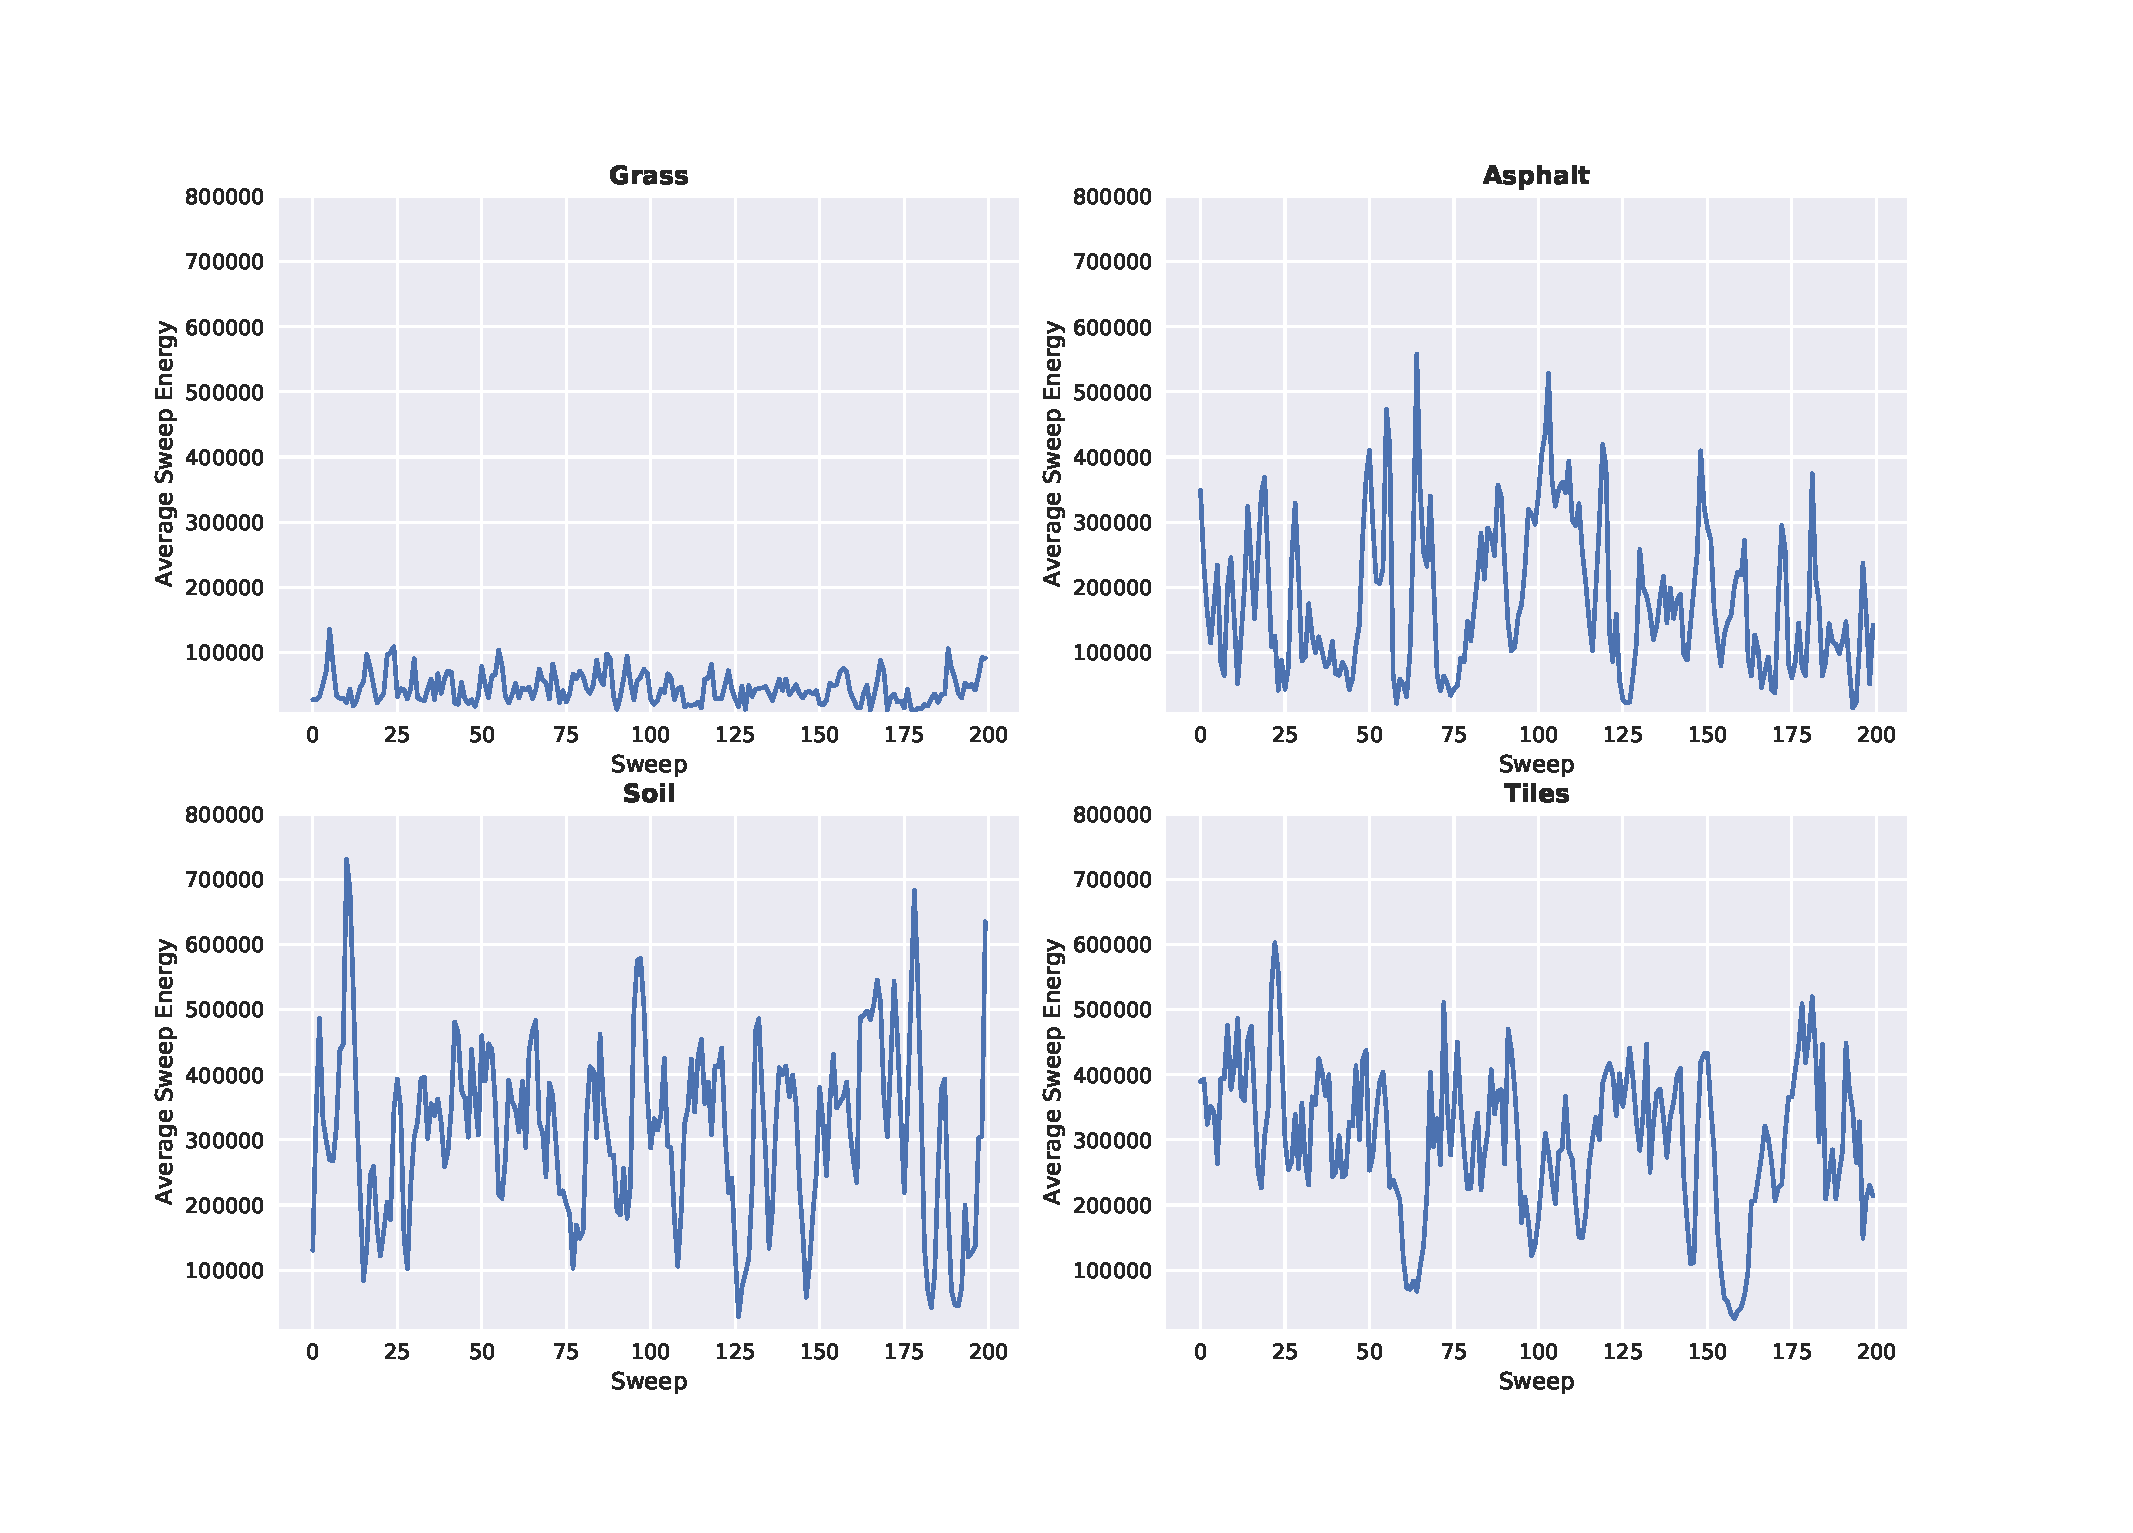
\includegraphics[scale=0.45]{figs_temp/features/sweep_energy}
	\caption{The figure shows the average sweep energy for 200 sweeps and four different materials. All measurements were made during a short period of time. The reflections from the grass surface carry noticeably less energy than those from the other surfaces. }
	\label{fig:sweep_energy}
\end{figure}



\subsubsection{Fourier Transform}
The surface underneath the radar can be assumed to be static, whereas the radar traverses the surface at a constant speed. This causes the radar to detect doppler frequencies. Depending on the surface's characteristics, the doppler frequencies may vary, (according to figure *Figure comparing reflections on a flat and rough terrain*?) and to visualize the frequency contents of different measured materials, the discrete Fourier transform is used. 

To compute the Fourier transform, a "box" consisting of $T$ sweeps is selected. Viewing this as a matrix with elements $X_{n,t}$, where $n$ denotes slow time, and $t$ fast time we can write a Fourier transform in slow time at range $r$, within this box as
\begin{equation}
	\mathbb{X}_k^{(r)} = \sum_{n=0}^{T-1}X_{n,r}\exp\Big[-2\pi i\frac{nk}{T}\Big] \quad k=0, ..., T-1.
\end{equation}
In figure \ref{fig:fft} five consecutive 128-step Fourier transforms have been computed for four materials. For grass (top plot), it can be seen that the frequency content is contained mainly at the start of the "FFT blocks", which corresponds to normalized frequency 0. The other materials contain slightly higher frequency content as well.

To avoid aliasing we refer to chapter earlier in report where this is discussed. Mention that $\mathbb{X}_k^{(r)}$, for all $r$, $k$, is flattened to a vector, resulting in one new sample.

\begin{figure}[h]
	\centering
	\includegraphics[scale=0.4]{figs_temp/features/fft}
	\caption{Each plot shows 5 concatenated DFTs, which have all been estimated from 128 consecutive sweeps. This has been done for ranges 7-23 cm, and the materials included in the figure are grass, asphalt, soil and tiles, respectively. Each FFT box has an $x$-axis going from normalized frequency 0 to 1.}
	\label{fig:fft}
\end{figure}





\rowcolors{2}{gray!25}{white}
\begin{table}
\begin{center}
  \begin{tabular}{|c|cccc|}
\hline
    \rowcolor{gray!150}
                  & \color{white}\textbf{Abs} & \color{white}\textbf{AC Energy} & \color{white}\textbf{AC Range} & \color{white}\textbf{FFT}\\
    Config 1 & X & & & \\
    Config 2 & X & X & X&\\
    Config 3 & & & &X\\
\hline
  \end{tabular}
\end{center}
\caption{Feature configurations}
\end{table}

\section{Mutual information}

In (link to information section) it was briefly discussed that information theory metrics can be utilized when considering which data is of interest. 

While a useful metric, estimating MI can be a non-trivial task. k-nearest neighbors introduced here:
\citep{kraskov_stögbauer_grassberger_2004}

The particular link between continuous features and discrete values that we use are itnroduced  here:
\citep{ross_2014}


% Classification schemes
\chapter{Classification schemes}

In this chapter a few classification models are evaluated for the feature extraction processes described in the preceding chapter. Detailed descriptions of each classification framework is omitted, but good sources for further explanation will be supplied for the interested reader. The aim of this chapter is to compare various models and to determine the most promising one with regards to accuracy, size and complexity. 

\section{Evaluated models}

In this section the effectiveness of a few different models are compared. Two linear models and two non-linear models are evaluated. The two linear models considered, a \emph{Linear Discriminant Analysis} (LDA) and a \emph{Support Vector Machine} (SVM) model.

\subsection{Deep neural networks}

Deep neural networks, or DNN for short, are neural networks that has more than one layer of hidden units between its inputs and outputs \citep{hinton_deng_yu_dahl_mohamed_jaitly_senior_vanhoucke_nguyen_sainath_2012}. 


DNN's in various forms have gained immense popularity over the past two decades achieving considerable success within a wide spectrum of applications, such as in image recognition \citep{szegedy_liu_jia_sermanet_reed_anguelov_erhan_vanhoucke_rabinovich_2018}, acoustic modeling of speech \citep{hinton_deng_yu_dahl_mohamed_jaitly_senior_vanhoucke_nguyen_sainath_2012}, 

\subsection{LSTM}
Mention CNN and LSTM being used for time series classification. Then bring up the article which combines these two to motivate this approach.

Observing one range bin at a time, one could think of the radar data as a time series. This motivates the use of some classification scheme that exploits temporal behaviour. Recurrent neral networks (RNNs) feature this by having feedback within individual layers in the network. \citep{karim_majumdar_darabi_chen_2018} The problem with RNNs, however, is that they suffer from a vanishing or exploding gradient, and can only sustain a short term memory. A way to combat this is to use a neural network layer called long short term memory (LSTM). These are thoroughly described in, for example \citep{hochreiter_schmidhuber_1997}

LSTM-layers have previously been used successfully for classifications in radar applications. For instance in \citep{jithesh_sagayaraj_srinivasa_2018} the method was able to classify flying objects from $\textbf{nnn}$ different classes with an accuracy of ...? In \citep{karim_majumdar_darabi_chen_2018}, the LSTM layer is used in combination with a fully convolutional neural network (FCN), which proves to be a significant improvement from just using FCNs when classifying time series.

% Define block styles
\tikzstyle{decision} = [diamond, draw, fill=blue!20, 
    text width=7.5em, text badly centered, inner sep=0pt]
\tikzstyle{block} = [rectangle, draw, fill=blue!20, 
    text width=7em, text centered, rounded corners, minimum height=4em]
\tikzstyle{line} = [draw, -latex']
\tikzstyle{cloud} = [draw, ellipse,fill=red!20, node distance=3cm,
    minimum height=4em]
\tikzstyle{blockgreen} = [rectangle, draw, fill=green!20, 
    text width=7em, text centered, rounded corners, minimum height=4em]
\tikzstyle{blockbrown} = [rectangle, draw, fill=brown!20, 
    text width=7em, text centered, rounded corners, minimum height=4em]

\begin{figure}
\centering
\begin{tikzpicture}[node distance = 3cm, auto]
	% Place nodes
	\node [blockbrown] (obtained) {Obtained data};
	\node [blockgreen, below left of=obtained] (training) {Training data};
	\node [block, below right of=obtained] (test) {Test data};
	\node [blockgreen, below of=training, node distance=2.2cm] (train pre) {Preprocess and extract features};
	\node [block, below of=test, node distance=2.2cm] (test pre) {Preprocess and extract features};
	\node [blockgreen, below right of=train pre] (est) {Estimate $\mathbf{\mu}_f$, $\mathbf{\sigma}_f$};
	\node [blockgreen, below left of=est] (scale train) {Scale to ZMUV};
	\node [block, below right of=est] (scale test) {Scale to ZMUV};
	\node [cloud, below right of=scale train] (train model) {Train model};
	\node [decision, below of=train model] (classify) {Classification};
	\node [block, below of=classify] (post) {Postprocessing};
	\node [block, below of=post, node distance=2.2cm] (output) {Model output};
	% Draw lines
	\path [line] (obtained) -| (training);
	\path [line] (obtained) -| (test);
	\path [line] (training) -- (train pre);
	\path [line] (test) -- (test pre);
	\path [line, dashed] (train pre) -| (est);
	\path [line,dashed] (est) -- (scale train);
	\path [line,dashed] (est) -- (scale test);
	\path [line] (test pre) -- (scale test);
	\path [line] (train pre) -- (scale train);
	\path [line] (scale train) |- (train model);
	\path [line] (train model) -- (classify);
	\path [line] (scale test) |- (classify);
	\path [line] (classify) -- (post);
	\path [line] (post) -- (output);
\end{tikzpicture}
\caption{Flowchart of classification scheme.}
\end{figure}

\section{Model evaluations}


% Put a common title, "Accuracy", for all models
\rowcolors{2}{gray!25}{white}
\begin{table}
\begin{center}
  \begin{tabular}{|l|l|}
    \rowcolor{blue!35}
Material & DNN \\
pgrass1& 98.25 \\
pgrass2& 88.25 \\
pgrass3& 100.0 \\
pgrass4& 94.7 \\
pgrass5& 97.9 \\
qgrass1& 95.75 \\
qgrass2& 98.4 \\
qgrass3& 99.95 \\
hgrass12& 97.25\\ 
hgrass2 &98.4 \\
hgrass3 &99.65 \\
hgrass4 &99.85 \\
hgrass5 &99.5 \\
hgrass6 &100.0 \\
hgrass7 &98.5 \\
hgrass8 &97.5 \\
hgrass9 &98.65 \\
hgrass10& 95.25\\ 
hgrass11& 96.55\\ 
pasph1 &100.0 \\
pgravel1& 98.15 \\
pasph2 &99.95 \\
pasph3 &99.9 \\
psoil1 &99.9 \\
psoil2 &99.15 \\
ptiles1& 97.8 \\
qasph1& 99.95 \\
qasph2& 100.0 \\
qgravel1& 97.15 \\
qsoil1 &99.9 \\
qsoil2& 94.05 \\
qtiles1& 99.55 \\
rtiles1 &99.9 \\
rgravel1& 99.35 \\
rgravel2 &99.35 \\
rasp1 &99.9 \\
rsoil1 &93.45 \\
G2gravel2& 99.65\\ 
G2gravel1& 99.8 \\
G2soil1 &94.3 \\
G2tiles1& 100.0 \\
hsoil1 &93.4 \\
hsoil2 &95.5
  \end{tabular}
\end{center}
\caption{Feature configurations}
\end{table}

\subsection{Evaluation metrics}

\subsubsection{Validation set accuracy}

\subsubsection{Leave-one-out accuracy}


% Postprocessing and optimization
\chapter{Postprocessing and optimization}

In the previous chapter a simple feed-forward neural network was found to be a suitable model for the surface classification problem investigated. In this chapter, some improvements and additions to this model are introduced. First, we perform some data augmentation to increase the number of training data. Then, removal of outliers using the clustering method DBSCAN is tested to see if accuracy can be further improved. Finally, two detection methods are discussed for outlier suppression.


\section{Data augmentation}

A recurring problem in training ANN's is that there simply isn't enough data \citep{lemley_bazrafkan_corcoran_2017}. Too little data will generate overfitting, which means that the network is highly biased to what it has seen in training and will subsequently perform poorly on any validation or test set. In the preceding chapter dropout was introduced for this particular purpose, and examining the cross validation accuracies it is clear that reasonable accuracy is attained without any further means.

However, by \emph{augmenting} the data we may be able to further increase the training set size, and subsequently further increase model performance. Data augmentation is the process of supplementing a dataset with similar data created from the same dataset. How one augments a dataset is of course data dependent. In computer vision, data augmentation often involves rotating, translating, blurring or in some other way modifying existing images \citep{lemley_bazrafkan_corcoran_2017}.

In the present case of increasing the number of data batches from a given data rectangle, we can simply allow for overlapping batches. Previously, when batches of length $T$ were generated from $Q$ slow time samples, every $T$ sweeps produced one batch providing a total of $Q/T$ batches for analysis. However, noting that any slow-time sequence of $T$ sweeps is a valid data batch, we may form overlapping batches from every $T/A$ samples, where $A$ is some integer factor selected so that $T/A$ becomes an integer. This produces $(A-1)(Q/T-1)$ additional batches providing a total $P$ batches of

\begin{equation}
	P = 
	\frac{Q}{T} + (A-1)\Big(\frac{Q}{T} - 1\Big) = 
	\frac{AQ}{T}-A+1.
\end{equation}


Setting $A=5$, one data rectangle consisting of 50,000 slow time samples normally yielding 2,000 data batches using $T=25$, instead produces 9996 data batches.  

----> Result here.

\section{Outlier removal}

In any dataset some data corruption is to be expected. A grassy surface may have small patches of soil without grass, the device may have been moving at either a too high or too low velocity for a short period of time or the radar sensor iteslf may have had temporary issues. Such processes forms data points inconsistent with the overwhelming bulk of data, or \emph{outliers}, which negatively impacts model performance. The importance of outliers is dependant both of their frequency and magnitude, and can be significantly detrimental to model accuracy making effective removal of them often necessary or at least benifitial \citep{osborne_overbay_2004}, \citep{hodge_austin_2004}. 

\section{Detection of surface change}

Even with an optimized model with tons of training data, erronous predictions are unavoidable in any real-world scenario. Prediction probabilities are produced by the model rapidly, 8 times a second for a sampling rate of 200 Hz and a batch size $T=25$ according to equation \ref{eq:classification_rate}. With such errors present in the prediction confidences of the model, what is a reasonable strategy to detect when a change in surface has occurred?  




Many elaborate statistically appealing methods for change detection are presented in \citep{basseville_nikiforov_1993}. These methods require some basic assumptions on the data it attempts to detect a change from, such as data having constant probability distribution before and after a parameter change occurs. This, however, renders these methods difficult to use in the present use case, as we are dealing with the output of a highly nonlinear artificial neural network producing predictions with unknown structure. This is reinforced by examining what the ANN outputs, see the top figure in \ref{fig:trans_tgtg}. Predictions remain extremely stable for long periods of time, with occasional outlying predictions every now and then. 



Instead, median filtering was used to suppress prediction outliers. Median filtering simply calculates the median of some length $L$ nearest predictions. 


\citep{yin_yang_gabbouj_neuvo_1996}
Nonlinear filter
"The success of median based filters is based on two intrinsic properties: edge preservation and efficient noise attenuation with robustness against impulsive-type noise."
"Neither property can be achieved by traditional linear filtering techniques."
"The median filter is the optimal is the optimal filter for biexponential noise."
"Median filtering discards temporal ordering"

The perhaps most effective way of suppressing data littered with outliers is through some form of median filtering. The regular form of a median filter simply takes the median of current and previous datapoints, resulting in an output significantly less sensitive to inconsistencies \citep{pearson_2002}. After median filtering a threshold can be utilized, leading to the following predictions for a filter length $L$

\begin{equation}
	P_i=0 \quad\text{if}\quad\text{median}\{p\}_{i-L+1}^i\leq\xi, 
	\quad \text{else} \quad P_i = 1
\end{equation}


\iffalse
\section{Postprocessing and detection}


\begin{figure}
	\includegraphics[scale=0.5]{figs_temp/detect_nothing}
	\label{fig:detect_no}
	\caption{Transition region with some outliers}
\end{figure}

\subsection{Thresholding}

The simplest possible detection algorithm is by setting a threshold $\xi$, and classifying below surface as either grass or non-grass depending on whether the prediction is above or below the set threshold. Denoting the resulting prediction as $P$ this detection algorithm is 

\begin{equation}
	P_i=0 \quad\text{if}\quad p_i\leq\xi, \quad
	\text{else} \quad P_i=1
\end{equation}

However, for this method to fail only a single incorrect prediction $p_i$ is required so the algorithm is extremely sensitive to any errors in $p$.

\begin{figure}
	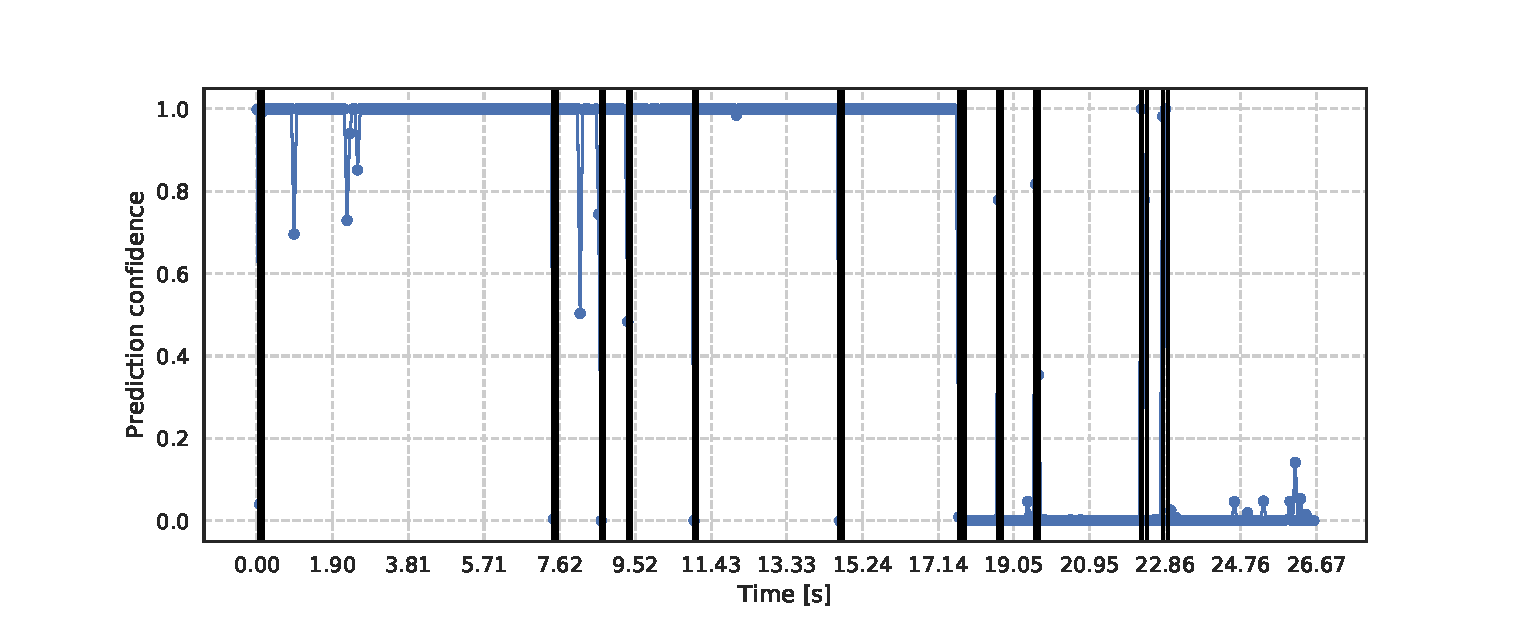
\includegraphics[scale=0.5]{figs_temp/detect_thresh}
	\label{fig:detect_thresh}
	\caption{Detecting transition region using thresholding.}
\end{figure}

\begin{figure}
	\includegraphics[scale=0.5]{figs_temp/detect_median}
	\label{fig:detect_median}
	\caption{Detection transition using median filtering}
\end{figure}

\subsection{CUSUM}

A traditional and statistically appealing method for effectively detecting abrupt changes in data is CUmulative SUM, hereby refered to as CUSUM. The cumulative sum computed in CUSUM is a log-likelihood $S$ defined through

\begin{equation}
	S_j^k = \sum_{i=j}^k \text{ln}\frac{p_{\theta_1}(y_i)}{p_{\theta_0}(y_i)}
\end{equation}

\begin{figure}
	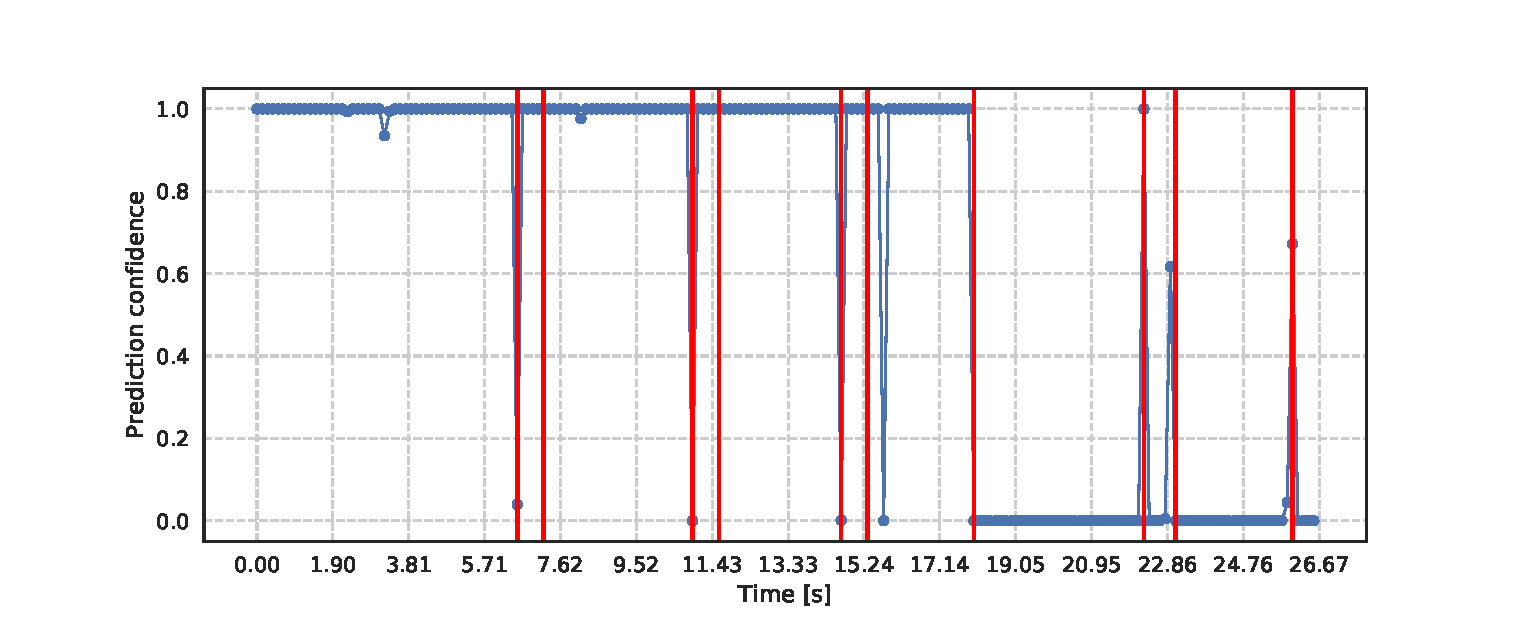
\includegraphics[scale=0.5]{figs_temp/detect_cusum}
	\label{fig:detect_cusum}
	\caption{Detection of transition using CUSUM.}
\end{figure}

[Continue explanation]






\subsection{Method comparison}

After introducing each detection algorithm a comparison is in order. Below is output from a typical transition using [model we made]. Each algorithm has been applied to the data for change detection.


Informal definition as data points inconsistent with our expectations

\section{Removal of outliers}


\subsection{Mahalanobis distance}

\subsection{DBSCAN}

\section{Hyperparameter optimization}
\fi




% Discussion
\chapter{Results and Discussion}
In this section the best models' capabilities are tested and discussed. Previously, the model has been evaluated on labeled data, providing a clear ground truth to evaluate the models predictions on. Below, the model will instead make predictions on unlabeled data, and instead output its confidence in its prediction. We then discuss various topics with regards to the results found and some overall considerations.

\section{Real and artificial transition regions}

While we up to this point mainly have focused on \gls{loo} accuracies we have not in detail studied what the neural network softmax output that we base our classification on looks like. We are specifically interested in examining how well performance is when the robot moves across a \emph{transition region}, a region where the surface type changes from grass to nongrass or vice versa. Ideally the prediction should rapidly change according to the new target surface. 

This can be accomplished in two different ways. The first revolves around creating a test set through concatenation of sequences of radar sweeps from a few different data matrices. By selecting alternating surface types we artificially generate transition region data which we can predict on. Examining these predictions we get a feel for what output the predictor may generate when moving from one surface to the next. The second method is to use real-world measurements from when the robot moves from one surface to the next. We should see that when the robot has reached the transition the prediction changes accordingly. 

\begin{figure}[t]
	\centering
	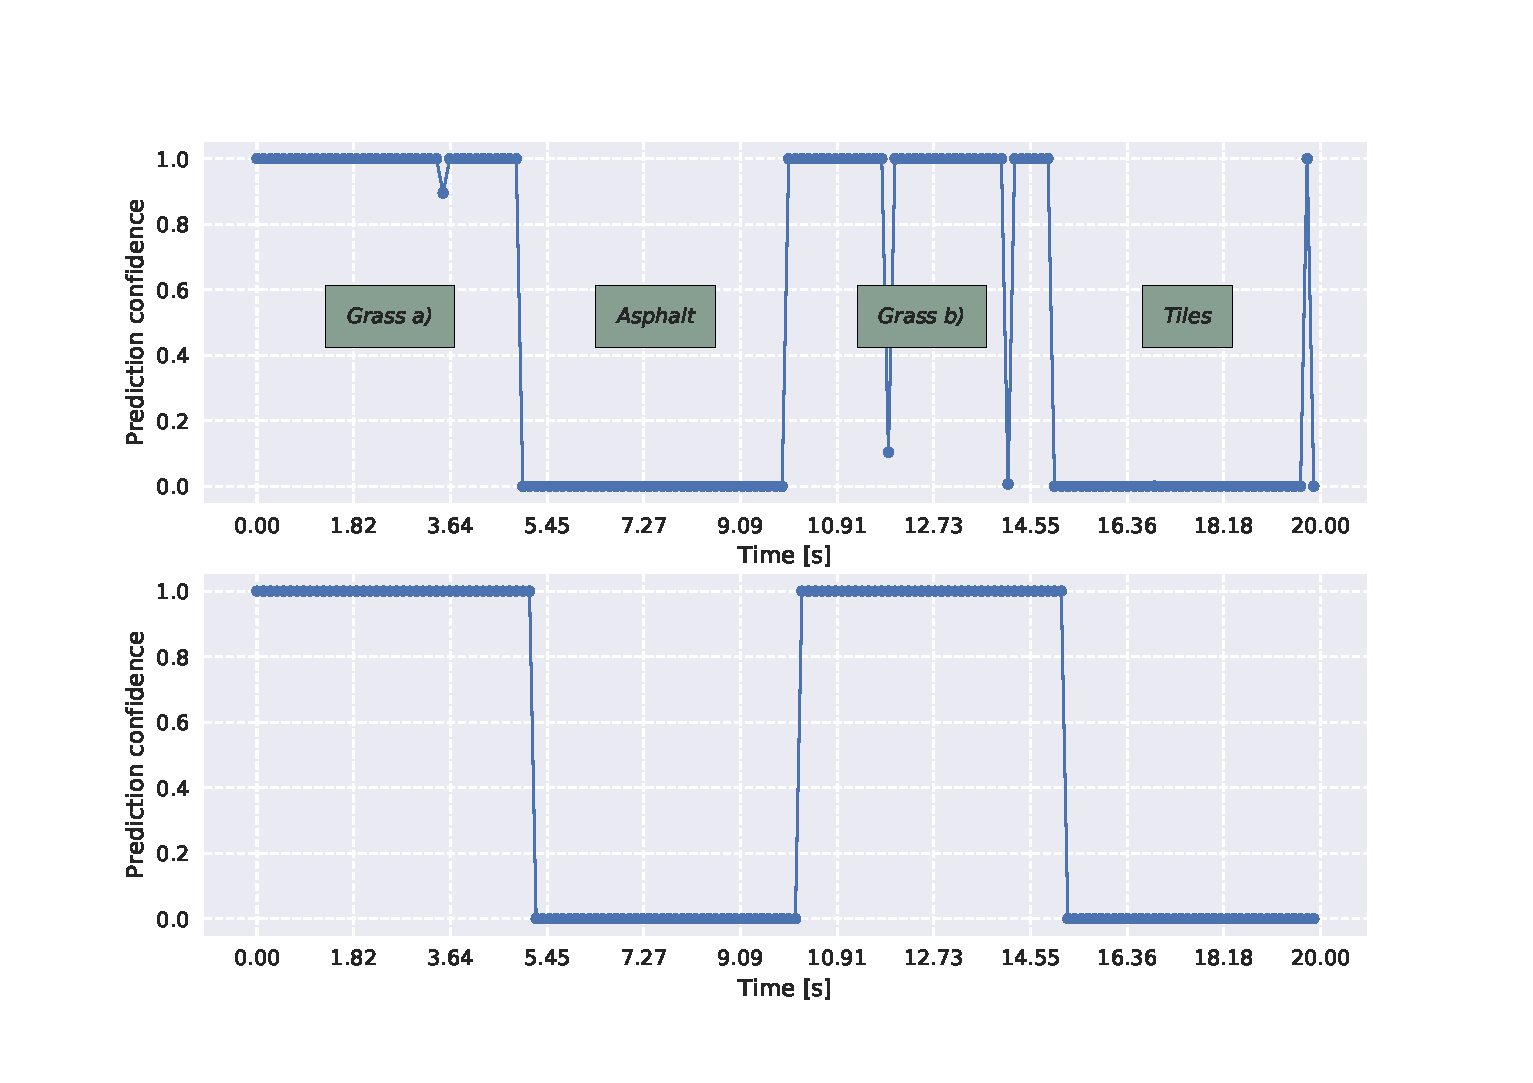
\includegraphics[scale=0.5]{figs_temp/varmats1}
	\caption{Predictions on an artificial transition region created using samples from four different regions. The bottom figure shows the median filtered predictions with filter length $L=5$.}
	\label{fig:artificial1}
\end{figure}

\begin{figure}[t]
	\centering
	\includegraphics[scale=0.5]{figs_temp/varmats2}
	\caption{Predictions on an artificial transition region created using samples from four different regions.}
	\label{fig:artificial2}
\end{figure}

In the first test, samples from four surfaces are concatenated into a sequence: grass, asphalt, grass and tiles, where the two grass samples were taken from different data matrices. The predictions are shown in the top part of figure \ref{fig:artificial1}. In the lower part of this figure, the predictions are median filtered with filter length $L=5$, see section \ref{surface_change}. The outliers are removed, rendering accurate predictions of the different surfaces. 

Two more challenging surfaces, according to table \ref{tab:loo}, are soil and gravel. In figure \ref{fig:artificial2} predictions on artificial transitions on these are shown. Something worth noting in the two figures is that the surface transition is delayed by two steps after the median filtering. It is important to be aware of what distance this corresponds to in the physical world, since we do not want to detect an edge long after it is passed. Each prediction uses 25 samples, and with a delay of two predictions this means a 50 sample delay. With the sampling rate at 200 Hz (see table \ref{tab:sensor_settings}), this means a 0.25 second delay in the edge detection, which for a robot traveling at the speed of $v=0.3$ m/s means a spatial delay of $0.3\cdot0.25=0.075$ m.

Looking at the high \gls{loo} accuracies in table \ref{tab:loo}, the results of classifications upon the artificial transitions should not come as a surprise, as they are based on the same data. What can be seen that we didn't know from table \ref{tab:loo} is that not only does the model classify correctly, but usually  does so with a very high confidence. 

To test the model further, data was collected when the test robot moved from one surface to another. Figure \ref{fig:trans_tgtg} shows a transition from grass to tiles, and figure \ref{fig:trans_gg} a transition from grass to gravel. Focusing on the median filtered predictions, we see that outside the transition region, the model works well for classifying either surface. Looking at the transitions sections, we see a rather sharp switch in prediction confidence. Nonetheless, this switch is not immediate. This is likely due to that the wide combined field of view of the two sensors (see figure \ref{fig:sensor_placement}) capturing both regions simultaneously, and thus try to predict data obtained from a mixture of the two. 

% I think this explanation is overly long
%What happens around the transition is perhaps more interesting. In the previous figures, the predictions went from 1 to 0 and vice versa in just one step. Here, it takes a while before the model reaches zero-outputs. There are two possible explanations for this. First of all, in the artificial transitions, the surface went from a perfect grass surface to a perfect non-grass surface at an instance. In real transitions, there might be some overlap of grass on the non-grass surface, making the model unsure of what it sees. Another explanation could be that one sensor is facing straight down, whereas the other one looks slightly more forward. Hence, the model is perceiving both grass and tiles simultaneously during a short time. 

% ?
%The results show great promise, but the work is still at an early stage. The surfaces in the four transitions were intentionally free from as many obstructions as possible. When facing surfaces with characteristics not taken into regard by the model, the results will not likely be as good. 
\begin{figure}
	\centering
	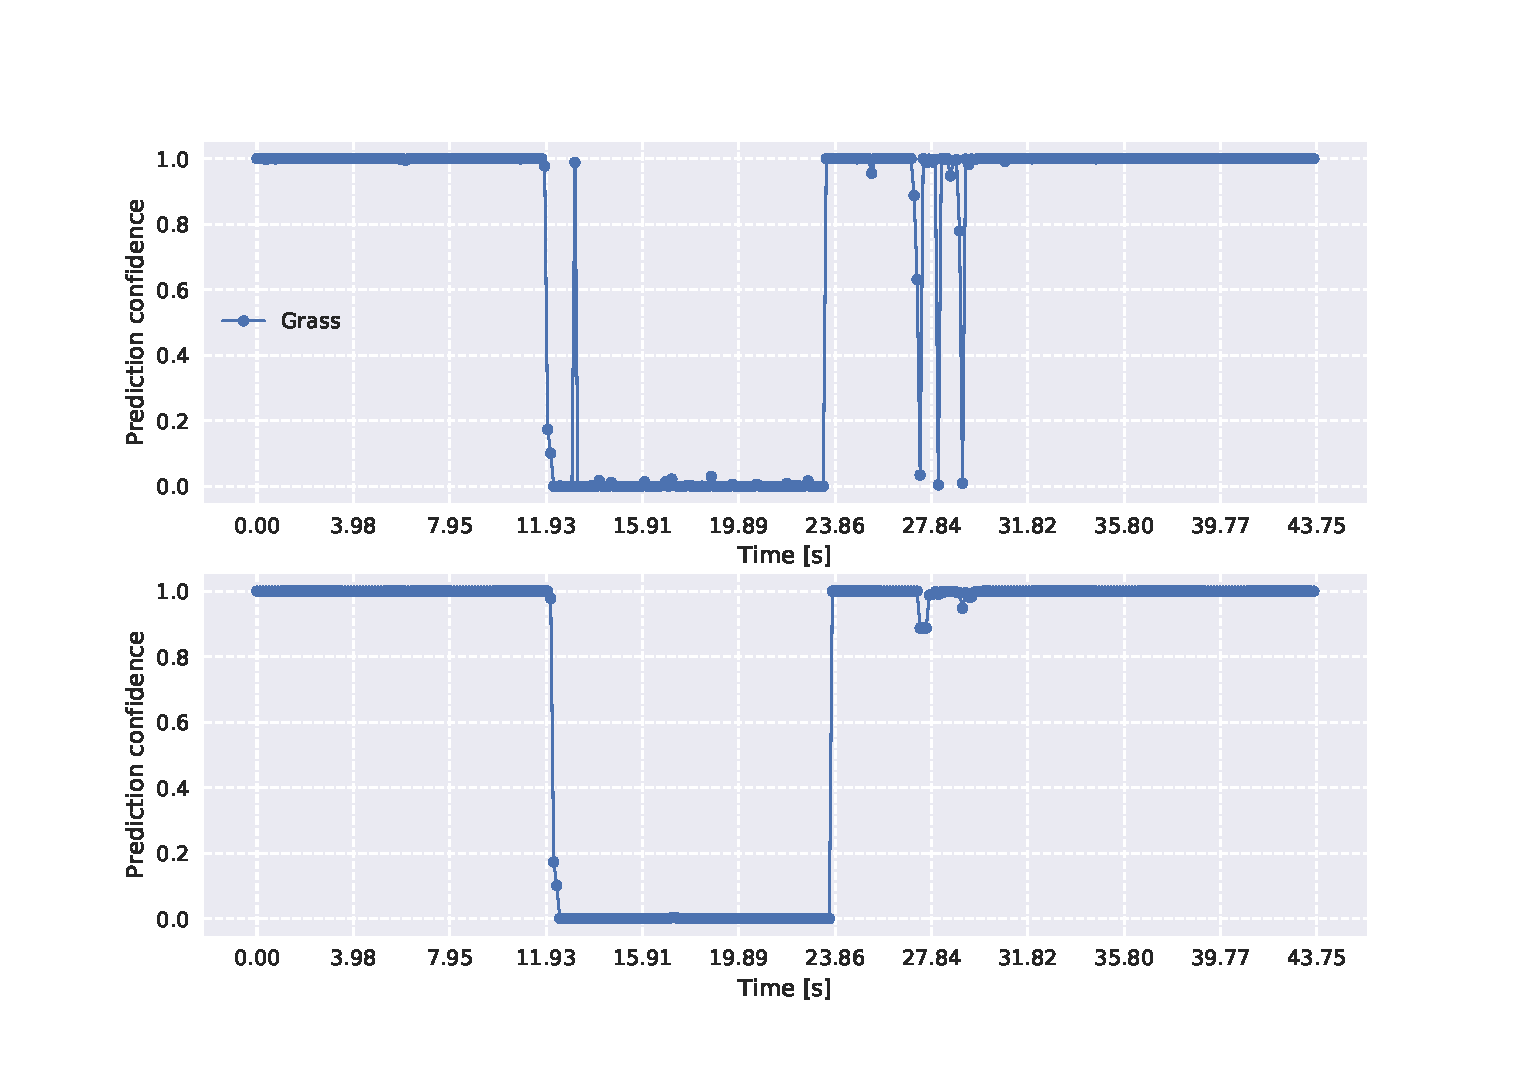
\includegraphics[scale=0.5]{figs_temp/transition_grass_tiles_grass}
	\caption{Predictions from a real-world test where the robot moved from grass to a tiled pavement.} 
	\label{fig:trans_tgtg}
\end{figure}

\begin{figure}
	\centering
	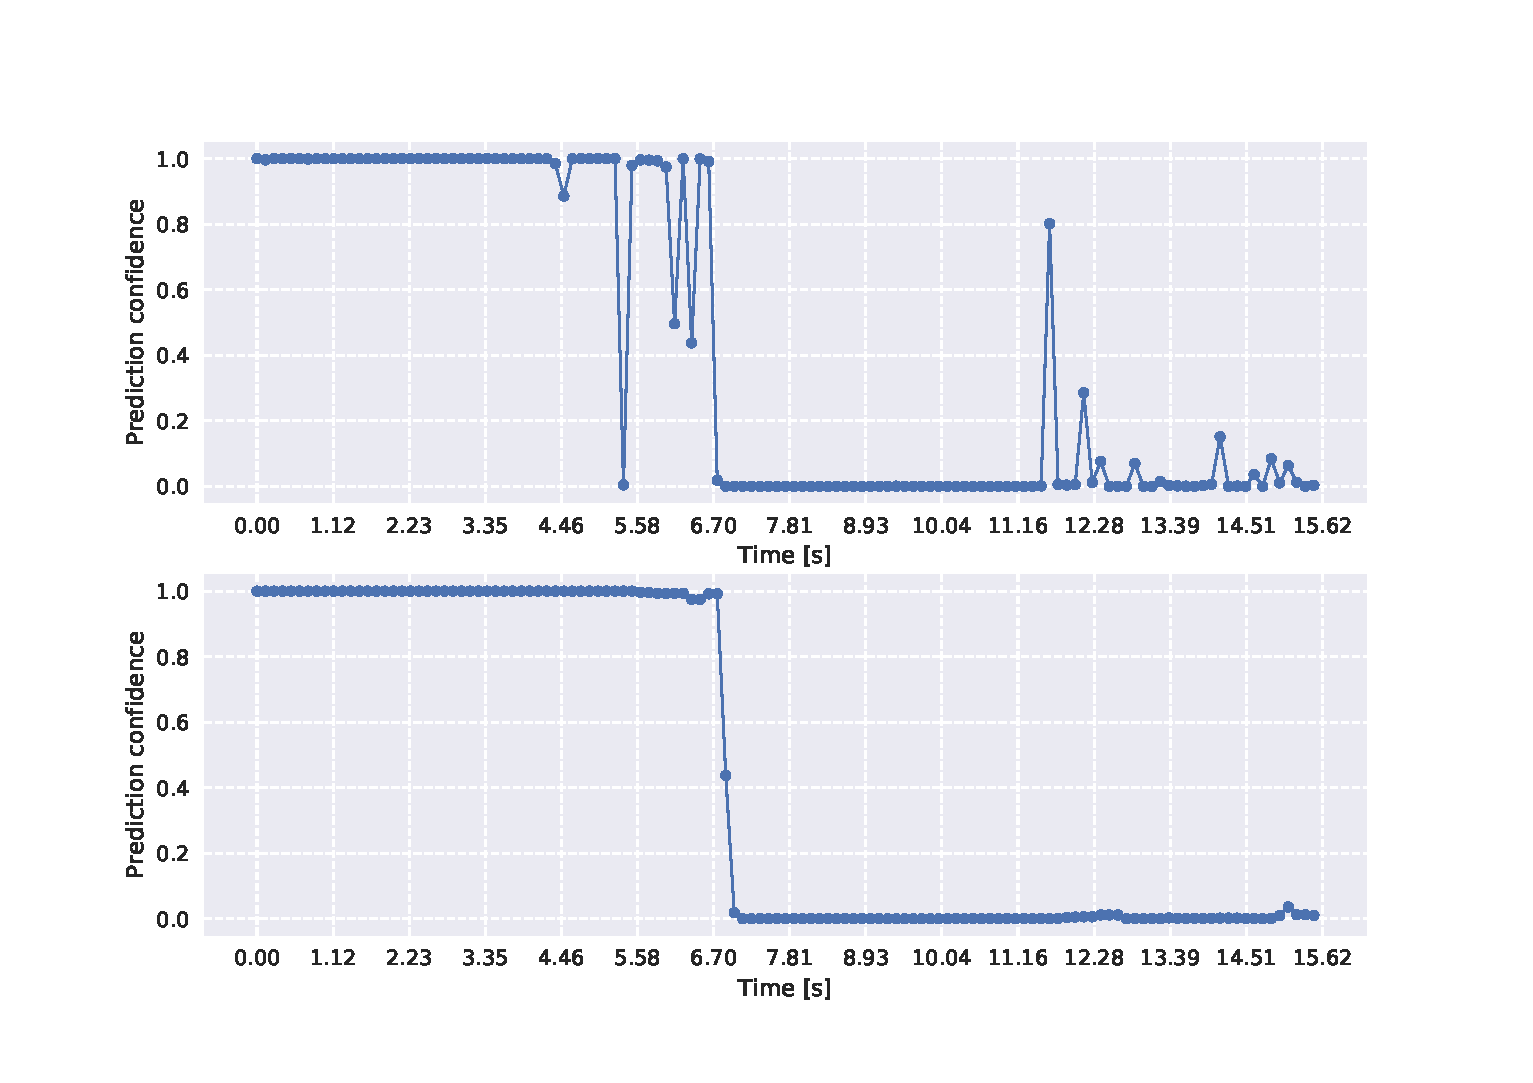
\includegraphics[scale=0.5]{figs_temp/transition_grass_gravel2}
	\caption{Predictions from a real-world test where the robot moved from grass to gravel.}
	\label{fig:trans_gg}
\end{figure}

\section{Surface Variances}

On particularly challenging aspect of adequately classifying surfaces, that was briefly touched upon in section \ref{sec:chall}, is that the space of realistically occurring surface variations is essentially infinite. As any lawn owner can testify a lawn changes drastically over the course of its life span depending on grass height, weather conditions, tear and temperature. One would certainly need an enormous training dataset to capture all such features. And that would still only account for one single lawn. 

However, we see from our results that accurate classification is possible when acquired data is reasonably similar to what has been seen in training. A robot \emph{can} learn to identify surfaces as being grassy or not provided that it has previously been exposed to somewhat similar surfaces before. 
%%%%%%%%%%%%%%% Introduce again when we actually have done it.
%\section{Difficult Surfaces}


%While we only have five material classes in this work, each class can be broken down to multiple subclasses. Taking grass as an example, it may vary in a wide range of attributes such as length, humidity and sparsity to name a few. Therefore it is important to gather a dataset as diverse as possible, so that the model has trained on all common varieties of each surface. 

%However, the model can only be prepared for so much, and an often critical aspect of any machine learning system is its performance on dissimilar data. It is difficult to foresee how a complex neural network will interpret a surface displaying characteristics not included in training. For instance, what would the model make of a lawn which is partially covered by leaves and twigs; or a surface type it has never seen before? Perfecting the model to work in any surrounding calls for a good sense of what difficulties may occur, as well as a large time investment. 




%\section{Moisture}

%One particularly challenging aspect of adequately classifying surfaces is the ever-changing environmental conditions surronding the sensor. Of particular interest is the moisture content in the surfaces of interest. Greater soil moisture implies higher dielectric constant, which in turn increases radar wave scattering \citep{rappaport_2006}. Thus a single surface may very well change its scattering properties over time. 

% More things that make selecting data tricky

%\section{Surface variances}


%Such effects is difficult to account for when selecting data. Gather a dataset as diverse as possible



\section{Feature Extraction and Model Selection}
\label{disc_feat}
Table \ref{tab:loo} is in many ways a very telling one. Using the \gls{loo} cross validation scheme each data measurement was classified without using any of the samples from the session at hand. Six different methods of classification were evaluated; two linear and four nonlinear. 

First and foremost it is noted that each tested method performed at the very least \emph{decently}. One may argue that the \gls{lstm} model is unstable or that using \gls{lda} produces lower accuracy predictions, but they nonetheless generated accuracies above 97\% on average. Considering these are the lower-performing classifiers, and the remaining ones perform even better, suggests that the performed feature extraction captures, or at least maintains, most of the cruicial information in the original data. Furthermore, as linear models managed to separate data decently we know that the information content in data is readily available without the usage of more advanced non linear classifiers.  

A deep learning puritan might argue that no feature extraction should be performed when working with deep neural networks; a network should be able to find good data characteristics on its own. Hence, and \gls{ann} may yield a better result by omitting the feature extraction as this unavoidably discard some information in the original data. However, since much of the information seems to be found in how signals evolve over time, a network with no feature extraction would require multiple sweeps to be concatenated into one feature vector in order to be able to find these time dependencies. Say it would take 25 (downsampled) sweeps, each with 14 range bins. Each sweep would then produce 28 features as the real and imaginary part are divided into separate features. The feature vector to such a network for two sensors with different mounting angles would then consist of $2\times25\times28=1400$ features. Furthermore the network would have to figure out all the complex-valued temporal processing techniques that we already know how to calculate from theory. So although using no feature extraction method whatsoever could \emph{potentially} increase accuracy with a large \gls{dnn} model, we argue that the added complexity and reduced control is a high price to pay for this increase. 

On a different note, the final choice of classifier is debatable. The \gls{dnn} classifier was chosen mainly due to its high stable \gls{loo} scores in table \ref{tab:loo}. Nonetheless linear models performed well too, but didn't quite reach the accuracies of the \gls{dnn} model, implying that the features are at least \emph{approximately} linearly separable. Placing more effort on the linear models through testing more types of lienar classifiers and optimizing their hyperparameters more carefully might make one of the linear models the top choice.

% TODO: Discuss the LSTM+CNN model

\section{Errors and Uncertainties}
% Not needed imo
%As with all works, there are things that can go wrong due to either technical reasons or human reliability. The data collecting process is a prime example of where human reliability is inevitable. Here, fundamental decisions are made, which the entire work is based upon. For instance, in general, one strives for a dataset where the numbers of samples from each class are as balanced as possible. 

For this project a total of 42 data matrices were captured from 5 different surfaces, see table \ref{tab:count}. The number of matrices acquired from each surface was based on having a reasonably balanced dataset with a similar number of grass and non-grass samples. Having a balanced (or near-balanced) measurement set ensures that the classification is not biased either way; with more samples of one class the classifier will naturally tend towards the surface type it has seen more of in training. This however leaves other surfaces with less similar training data, and it is well possible that more measurements of the lower-performing soil and gravel surfaces are needed.  

% I think this is weirdly written
%But the question of what a balanced dataset \emph{is} sometimes holds multiple answers. In this work, there are four different types of materials belonging to class 0 (not grass) and one belonging to class 1. A natural question to ask oneself is whether there should be equally many samples for each \textit{material}, or equally many for each \textit{class}. We have chosen to balance the dataset so that there are approximately as many samples in each class. If all grass surfaces looked the same, this would perhaps make the model biased in its predictions, but due to the great variety among grass surfaces the bias is eliminated.

Another risk when collecting data is obtaining too little of it. By looking at how little improvement the data augmentation made, it would seem that obtaining $Q=50,000$ sweeps per measurement session and data matrix was enough. However by increasing the number of data matrices collected we increase \emph{data diversity}, capturing a wider range of grass types. 

A more technical uncertainty regards the assumption of a constant velocity over different surfaces. The robot used in this project kept a somewhat steady pace regardless of surface type, but when faced with rough terrain or steep hills the robots velocity altered a fair bit. As both the \gls{dft} and autocovariance require a consistency in the spacing between sample points, we cannot tolerate too large variations in velocity. Hence, to sample at regular distaces the sampling could be controlled by positional feedback from the robot rather than a fixed sampling frequency.

% TODO: I think this should either be moved to future work or not included
% While this work has not put much focus on \textit{live} classifications, this does pose a new limitation on the model. Ideally we want the system to collect $T$ samples, and make an instantaneous prediction so that $T$ new samples can be collected right away. By running the system on a single thread, however, the time it takes to generate a prediction delays the data collecting process with some time $t_{cl}$, as only one process can be ran at a time. An alternative could be to handle the classifications in a separate thread. That way, data could be collected continously, while classifications are performed in parallel. Doing this requires caution. If the time it takes to generate a classification exceeds the time it takes to collect $T$ samples, i.e. $t_{cl}>T/F_s$, a delay will accumulate over time. After a while predictions would be irrelevant as they would be based on surfaces far behind the robot. A natural limitation to assign the model is therefore
%\begin{equation}
%	t_{cl} \le \frac{T}{F_s}.
%\end{equation}
%The time $t_{cl}$ has not been discussed in this work, but is highly relevant to study in the future.



% This remarkable result means that given a random sample from the dataset collected, with no samples from the session the sample was taken from used in training, we can correcly classify the surface as grass or non-grass 39/40 times even with the lower-performing classifiers. With the top performing fully connected model, even higher accuracy was obtained with a low standard deviation. 




% Conclusions and future work
\chapter{Conclusions and Future Work}

\section{Conclusions}
In this work, the possibilities of using millimeter-wave radar for surface classification were explored. We found that by manually extracting features exploiting temporal behaviour and combining this with a deep neural network model, we were able to perform binary classification, distinguishing grass-surfaces from other types of surfaces with an accuracy as high as 98.5 \%. Using a median filter, predictions were improved, giving a perect result on test data, as well as a promising result on basic real world applications. When confronted with unfamiliar surfaces, the model falls short, and further investigation in this area is required. 
% Mention that patent application has been submitted. Ask Peter how this ought to be phrased and what to include?


\section{Future work}

	No feature extraction
	Automatic feature extraction(/selection?)
	More data! And more types of data
	Test for other tasks - such as road condition monitoring
	Implement velocity-dependent sampling rate
	Linear and non-linear models
	Outlier removal


% Appendices


\begin{appendices}

	\chapter{IQ Demodulation}
	IQ demodulation is a major part in the receiver processing of radar data. When an echo produced by a single scatterer is received by the radar, it can be described as
\begin{equation}
\label{eq:signal}
	x_R(t)=A(t)\sin(\Omega t+\theta(t)).
\end{equation}
Here, $\Omega$ is the carrier frequency of the transmitted pulse and the time, $t$, relates to distance according to equation \textbf{*ref*}. The goal of IQ demodulation is to extract $A(t)$ and $\theta(t)$ from \eqref{eq:signal}, and end up with a complex signal of the form $A(t)e^{i\theta(t)}$.

Most classical radars follow the demodulation scheme depicted in figure *ref*. The first step is to split the signal in \eqref{eq:signal} into two separate channels. In the upper channel, the signal is multiplied by a sinusoid which is generated with the same carrier frequency as the received pulse. The result of this multiplication can be rewritten as
\begin{gather}
	 A(t)\sin(\Omega t+\theta(t))\cdot 2\sin(\Omega t) = \\
	\label{eq:split}
 	 A(t)\cos(\theta(t))-A(t)\cos(2\Omega t+\theta(t)).
\end{gather}
The next step in the demodulation scheme is to low pass filter the signal. Thus, the high frequency term in \eqref{eq:split} is removed, and only $A(t)\cos(\theta(t))$ remains. We define this as $I(t)$.

Similarly, in the bottom channel in figure *ref to schematics*, the original signal is multiplied by a generated wave signal of the same carrier frequency. However, this time, the signal is shifted 90 degrees in phase. Just as before, we may rewrite the product as
\begin{gather}
	 A(t)\sin(\Omega t+\theta(t))\cdot 2\cos(\Omega t) = \\
	\label{eq:split}
 	 A(t)\sin(\theta(t))+A(t)\sin(2\Omega t+\theta(t)).
\end{gather}
After low pass filtering we obtain $A(t)\sin(\theta(t))$, which we define as $Q(t)$. Finally, by defining $I$ and $Q$ as the real- and imaginary parts of a complex number, respectively, we have our IQ-data
\begin{equation}
	I(t)+iQ(t)=A(t)\Big(\cos(\theta(t))+i\sin(\theta(t))\Big)=A(t)e^{i\theta(t)}
\end{equation}

\end{appendices}

\bibliography{refs}
\bibliographystyle{apalike}
\end{document}
